\chapter{Rezultati}
U jednom od poglavlja teksta, kako već ide konkretna struktura rada, nakon definiranja
modela uobičajeno se navode rezultati. Bilo da se radi o numeričkim,
eksperimentalnim rezultatima, rezultatima primjene neke analitičke metode ili
rezultatima procesa konstruiranja i sl.

\section{Prikaz rezultata}

\begin{figure}[H]
  \centering
  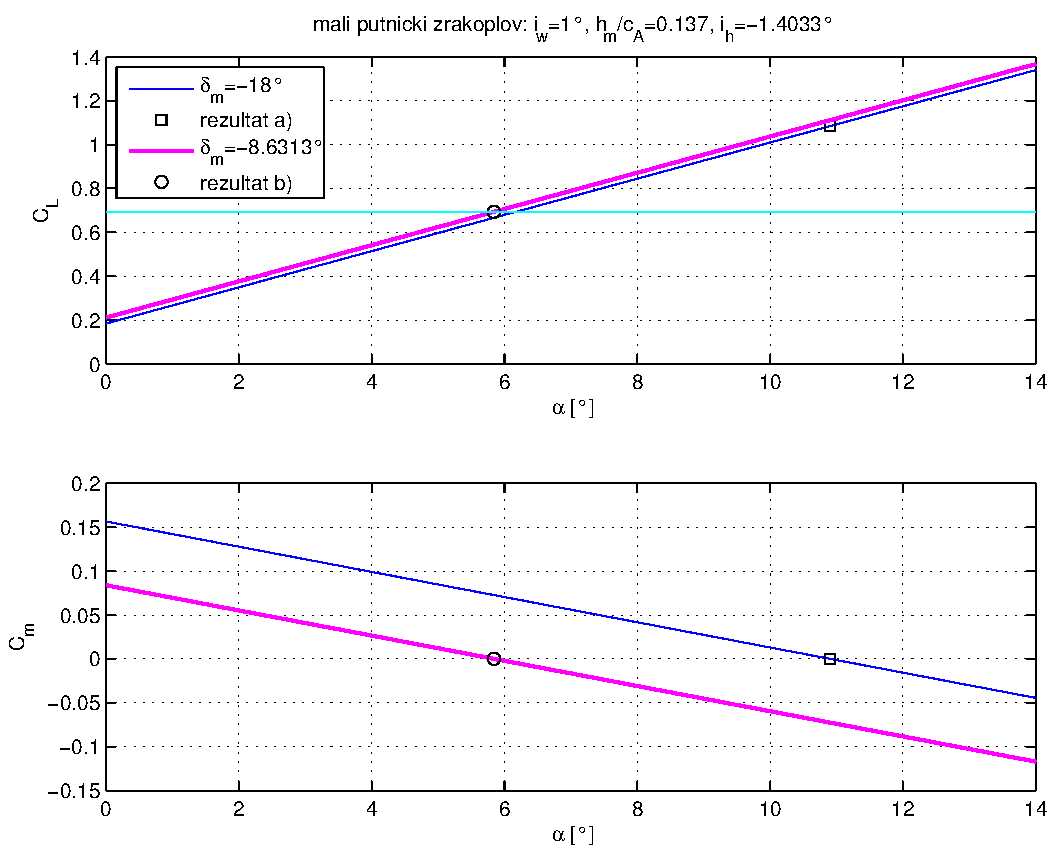
\includegraphics[width=0.95\textwidth]{03_Rezultati/rezultat}\\
  \hangcaption{Primjer prikaza rezultat: ako neka oznaka/krivulja/podatak sa
  slike nije opisan na samoj slici može ga se opisati u ovom zaglavlju;
  napomena: $C_L$ i $C_m$ su bezdimenzionalne veličine}
  \label{fig:rez}
\end{figure}

Pri prikazu rezultata (kao npr. na slici~\ref{fig:rez}) nužno je obratiti pažnju na
jednoznačno označavanje, kako veličina koje se prikazuju tako i njenih
jedinica (koje bi trebale biti u skladu sa SI sustavom, u rijetkim slučajevima
i po potrebi uz njih moguće je dodati i neke druge 
jedinice koje su uvriježene u praksi, kao npr. imperijalne jedinice u
zrakoplovstvu). Isto tako, za slučaj prikaza rezultata više varijabli
i/ili u više varijanti potrebno ih je sve označiti na samoj slici ili u njenom
zaglavlju. 

\nomenclature[acl]{$C_L$}{koeficijent uzgona uzgona letjelice}%
\nomenclature[acm]{$C_m$}{koeficijent momenta propinjanja}%
